\ifx\allfiles\undefined
\usepackage[dvipsnames]{xcolor}
\usepackage{amsmath}   % 数学公式
\usepackage{amsthm}    % 定理环境
\usepackage{amssymb}   % 更多公式符号
\usepackage{graphicx}  
\usepackage{wrapfig}   % 插图
\usepackage{mathrsfs}  % 数学字体
\usepackage{physics}   % 物理符号
\usepackage{booktabs}
\usepackage{tabularx}
\usepackage{longtable} % 支持跨页表格
\usepackage{array}     % 增强表格功能
\usepackage{multirow}
\usepackage{tikz}
\usepackage{tikz-3dplot} % 引入 tikz-3dplot 宏包
\usepackage{subcaption} % 用于子图排版
\usetikzlibrary{arrows.meta, positioning, shapes.geometric}
\usepackage{enumitem}  % 列表
\usepackage{geometry}  % 页面调整
\usepackage{ragged2e}
\usepackage{unicode-math}
\usepackage[hidelinks,
colorlinks=true,
allcolors=blue,
pdfstartview=Fit,
breaklinks=true]{hyperref}

\graphicspath{ {flg/},{../flg/}, {config/}, {../config/} }  % 配置图形文件检索目录
\linespread{1.5} % 行高

% 页码设置
\geometry{top=25.4mm,bottom=25.4mm,left=20mm,right=20mm,headheight=2.17cm,headsep=4mm,footskip=12mm}

% 设置列表环境的上下间距
\setenumerate[1]{itemsep=5pt,partopsep=0pt,parsep=\parskip,topsep=5pt}
\setitemize[1]{itemsep=5pt,partopsep=0pt,parsep=\parskip,topsep=5pt}
\setdescription{itemsep=5pt,partopsep=0pt,parsep=\parskip,topsep=5pt}

% 定理环境
% ########## 定理环境 start ####################################
\theoremstyle{definition}
\newtheorem{defn}{\indent 定义}[section]

\newtheorem{add}{\indent 补充}[section]

\newtheorem{lemma}{\indent 引理}[section]    % 引理 定理 推论 准则 共用一个编号计数
\newtheorem{thm}[lemma]{\indent 定理}
\newtheorem{corollary}[lemma]{\indent 推论}
\newtheorem{criterion}[lemma]{\indent 准则}

\newtheorem{proposition}{\indent 命题}[section]
\newtheorem{example}{\indent \color{SeaGreen}{例}}[section] % 绿色文字的 例 ,不需要就去除\color{SeaGreen}{}
\newtheorem*{zhu}{\indent 注}

% 两种方式定义中文的 证明 和 解 的环境:
% 缺点:\qedhere 命令将会失效【技术有限,暂时无法解决】
\renewenvironment{proof}{\par\textbf{证明:}\;}{\qed\par}
\newenvironment{solution}{\par{\textbf{解:}}\;}{\qed\par}
\newenvironment{yzh}{\par{\textbf{已知:}}\;}{}
\newenvironment{tui}{\par{\textbf{推导:}}\;}{\qed\par}

% 缺点:\bf 是过时命令,可以用 textb f等替代,但编译会有关于字体的警告,不过不影响使用【技术有限,暂时无法解决】

% ######### 定理环境 end  #####################################

% ↓↓↓↓↓↓↓↓↓↓↓↓↓↓↓↓↓ 以下是自定义的命令  ↓↓↓↓↓↓↓↓↓↓↓↓↓↓↓↓

% 用于调整表格的高度  使用 \hline\xrowht{25pt}
\newcommand{\xrowht}[2][0]{\addstackgap[.5\dimexpr#2\relax]{\vphantom{#1}}}

% 表格环境内长内容换行
\newcommand{\tabincell}[2]{\begin{tabular}{@{}#1@{}}#2\end{tabular}}

% 使用\linespread{1.5} 之后 cases 环境的行高也会改变,重新定义一个 ca 环境可以自动控制 cases 环境行高
\newenvironment{ca}[1][1]{\linespread{#1} \selectfont \begin{cases}}{\end{cases}}
% 和上面一样
\newenvironment{vx}[1][1]{\linespread{#1} \selectfont \begin{vmatrix}}{\end{vmatrix}}

\def\d{\textup{d}} % 直立体 d 用于微分符号 dx
\def\R{\mathbb{R}} % 实数域
%\newcommand{\bs}[1]{\boldsymbol{#1}}    % 加粗,常用于向量
%\newcommand{\ora}[1]{\overrightarrow{#1}} % 向量

% 数学 平行 符号
\newcommand{\pll}{\kern 0.56em/\kern -0.8em /\kern 0.56em}
\newcommand{\pa}{\partial}
\newcommand{\vvec}{\overset{\rightharpoonup\!\!\!\! \rightharpoonup}}
% 中文平行 parallel
\newcommand*\zhparallel{%
  \mathrel{\text{\tikz[baseline,line cap=round] \draw (0em,-0.3ex) -- (.4em,1.7ex) (.2em,-0.3ex) -- (.6em,1.7ex);}}%
}
\newcommand{\X}{\mathtt{X}}
\newcommand{\mT}{\raisebox{0.1ex}{$\scriptstyle -T$}} % 调整高度为 0.1ex
\newcommand{\lmT}{\raisebox{-0.85ex}{$\scriptstyle -T$}} % 调整高度为 -0.85ex
\newcommand{\mone}{\raisebox{0.1ex}{$\scriptstyle -1$}} % 调整高度为 0.1ex
\newcommand{\lmone}{\raisebox{-0.85ex}{$\scriptstyle -1$}} % 调整高度为 -0.85ex
\newcommand{\vsup}[1]{\raisebox{-0.1ex}{$\scriptstyle #1$}}
\newcommand{\lsup}[1]{\raisebox{-0.85ex}{$\scriptstyle #1$}}
\newcommand{\mathminus}{\!\!-\!\!} % 数学环境连字符



\begin{document}
% \title{\Huge{\textbf{赵爹《连续介质力学》笔记}}}
\author{作者:无名氏马}
\date{\today}
\maketitle                   % 在单独的标题页上生成一个标题

\thispagestyle{empty}        % 前言页面不使用页码
\begin{center}
    \Huge\textbf{前言}
\end{center}

    本笔记根据
    \href{https://www.bilibili.com/video/BV1c54y1W78q/?spm_id_from=333.1387.upload.video_card.click&vd_source=0745441b4a83ceba73d32af3b7b0a955}{赵亚溥老师2020年春季《连续介质力学》课程}
    和教材
    (赵亚溥. 理性力学教程. 北京: 科学出版社, 2020.)整理而成,仅供参考学习。

\begin{flushright}
    \begin{tabular}{c}
        \today
    \end{tabular}
\end{flushright}

\newpage                      % 新的一页
\pagestyle{plain}             % 设置页眉和页脚的排版方式(plain:页眉是空的,页脚只包含一个居中的页码)
\setcounter{page}{1}          % 重新定义页码从第一页开始
\pagenumbering{Roman}         % 使用大写的罗马数字作为页码
\tableofcontents              % 生成目录

\newpage                      % 以下是正文
\pagestyle{plain}
\setcounter{page}{1}          % 使用阿拉伯数字作为页码
\pagenumbering{arabic}
% \setcounter{chapter}{-1}    % 设置 -1 可作为第零章绪论从第零章开始
 % 单独编译时,其实不用编译封面目录之类的,如需要不注释这句即可
\else
\fi
%  ↓↓↓↓↓↓↓↓↓↓↓↓↓↓↓↓↓↓↓↓↓↓↓↓↓↓↓↓ 正文部分
\chapter{流体基本流动}
\section{class 17}
\begin{add}
    \textbf{此部分内容AIGC}

    普朗特学派是流体力学领域的重要分支,其核心成员包括August Otto Föppl、Ludwig Prandtl和Theodore von Kármán。他们共同建立了这一学派,并对流体力学的发展做出了深远贡献。
    
    \paragraph{August Otto Föppl}
    
    August Otto Föppl是普朗特学派的创始人之一,他的研究主要集中在力学和流体力学领域。Föppl的主要贡献包括在压力力学和弹性力学方面的研究,他提出了Föppl定律,该定律用于描述圆柱壳的形变。Föppl还积极推动了流体力学的发展,并与Ludwig Prandtl有着密切的学术交流。
    
    \paragraph{Ludwig Prandtl}
    
    Ludwig Prandtl被誉为流体动力学的先驱,他的研究深刻影响了整个流体力学领域。Prandtl提出了流体力学的基本方程,特别是Prandtl定律,该定律描述了流体流动的压力梯度与速度梯度之间的关系。
    此外,他还研究了气体动力学和旋转流体力学,Prandtl的理论为后来的流体力学研究奠定了基础。Prandtl的主要师从August Otto Föppl学习,他在Föppl的指导下完成了博士学位,并在之后的学术生涯中继承并发展了Föppl的研究方向。
    
    \paragraph{Theodore von Kármán}
    
    Theodore von Kármán是理论流体力学的奠基人之一,他的研究涵盖了流体力学、气体动力学和高速度流体力学。Kármán提出了Kármán-Weisbach方程,该方程用于描述粘性流体在管道中的流动。他的实验研究和理论分析为航空工程和流体力学的实际应用提供了重要依据。Kármán曾在Ludwig Prandtl的指导下完成博士学位,并在Prandtl的学术团队中进行了深入的流体力学研究。
    
    \paragraph{师生关系}
    
    \paragraph{Ludwig Prandtl的师从}
    
    Ludwig Prandtl在学术生涯的早期接受了August Otto Föppl的指导。在Föppl的课题组中,Prandtl接触了流体力学的基础理论,并在Föppl的支持下完成了博士学位论文。Föppl的学术风格和对流体力学的深刻理解对Prandtl的学术发展起到了关键作用。
    
    \paragraph{Theodore von Kármán的师从}
    
    Theodore von Kármán则是Ludwig Prandtl的重要学生之一。在Prandtl的指导下,Kármán深入研究了流体力学的理论问题,并在Prandtl的实验室中进行了大量实验研究。Kármán的学术成就在很大程度上得益于Prandtl的指导和学术环境。
    
    \paragraph{学术传承}
    
    August Otto Föppl、Ludwig Prandtl和Theodore von Kármán三人之间不仅存在师生关系,还形成了一个紧密的学术团队。Prandtl继承了Föppl的研究方向,并培养了Kármán等一批优秀的流体力学学者。这种跨代的学术传承使得普朗特学派的理论体系得以延续和发展,成为流体力学研究的重要基石。
    
    \paragraph{整体影响与意义}
    
    这三位科学家共同奠定了流体力学的基础,他们的研究不仅推动了学术领域的发展,也为工业和工程实践提供了重要理论支持。普朗特学派的建立标志着流体力学进入了一个新的阶段,其影响力至今仍在流体力学研究中发挥重要作用。
    \end{add}
    \begin{example}
        固体力学与流体力学的联系与区别

    \begin{center}
        \textbf{联系}
    \end{center}
    \subsubsection{连续介质假设}
    二者均基于连续介质假设,忽略微观结构细节,用连续场(如位移场、速度场)描述宏观行为。   
    \subsubsection{守恒定律}
    \begin{itemize}
        \item \textbf{质量守恒}:固体力学中隐含于物质坐标;流体力学中显式表达为$\frac{\partial \rho}{\partial t} + \nabla \cdot (\rho \vec{v}) = 0$
        \item \textbf{动量守恒}:共用Cauchy动量方程 $\rho \frac{D\vec{v}}{Dt} = \nabla \cdot \vec{\vec{\sigma}} + \vec{f}$
        \item \textbf{能量守恒}:均需考虑机械能与热能的转换
    \end{itemize}
    \newpage
    \begin{center}
        \textbf{区别}
    \end{center}

    \subsubsection{基本观点}
    \begin{table}[h]
        \centering
        \begin{tabular}{lcc}
            \toprule
            特征 & 固体力学 & 流体力学 \\
            \midrule
            研究对象 & 固体(晶体、聚合物等) & 流体(气体、液体) \\
            变形特性 & 有限变形可恢复(弹性) & 无限变形不可逆 \\
            描述方法 & 拉格朗日描述 & 欧拉描述 \\
            典型现象 & 应力集中、疲劳断裂 & 湍流、边界层分离 \\
            \bottomrule
        \end{tabular}
    \end{table}
    
    \subsubsection{本构关系}
    \paragraph{固体力学(以线弹性体为例)}
    广义胡克定律:
    \begin{align*}
        \vec{\vec{\sigma}} &= \vec{\vec{C}} : \vec{\vec{\epsilon}} \\
        \sigma_{ij} &= C_{ijkl} \epsilon_{kl}
    \end{align*}
    其中,$\vec{\vec{C}}$ 为\textbf{弹性张量},描述材料的弹性性质,其分量 $C_{ijkl}$ 表示材料在不同方向上的刚度。对于各向同性材料,弹性张量可简化为:
\begin{equation*}
    \sigma_{ij} = \lambda \epsilon_{kk}\delta_{ij} + 2\mu \epsilon_{ij}
\end{equation*}
其中 $\epsilon_{ij} = \frac{1}{2}\left(\frac{\partial u_j}{\partial x_i} + \frac{\partial u_i}{\partial x_j}\right)$ 为\textbf{应变张量},描述固体的变形。

    \paragraph{流体力学(以牛顿流体为例)}
    本构方程:
    \begin{equation*}
        \vec{\vec{\sigma}} = -p\vec{\vec{I}} + 2\mu \vec{\vec{D}} + \lambda (\text{tr}\vec{\vec{D}})\vec{\vec{I}}
    \end{equation*}
    应变率张量:
    \begin{equation*}
        D_{ij} = \frac{1}{2}\left(\frac{\partial v_j}{\partial x_i} + \frac{\partial v_i}{\partial x_j}\right)
    \end{equation*}
    其中,$\vec{\vec{D}}$ 为\textbf{应变率张量},描述流体的变形速率,其分量为:
\begin{equation*}
    D_{ij} = \frac{1}{2}\left(\frac{\partial v_j}{\partial x_i} + \frac{\partial v_i}{\partial x_j}\right)
\end{equation*}
    对不可压缩流体($\nabla \cdot \vec{v}=0$)简化为:
    \begin{equation*}
        \sigma_{ij} = -p\delta_{ij} + 2\mu D_{ij}
    \end{equation*}
    
    \subsubsection{控制方程对比}
    \paragraph{固体力学(Lam$\acute{e}$-Navier方程)}
    \begin{equation*}
        \rho \frac{\partial^2 \vec{v}}{\partial t^2} = \mu \nabla^2 \vec{v} + (\lambda+\mu)\nabla(\nabla \cdot \vec{v}) + \vec{f}
    \end{equation*}
    
    \paragraph{流体力学(Navier-Stokes方程)}
    \begin{align*}
        \rho \left( \frac{\partial \vec{v}}{\partial t} + (\vec{v} \cdot \nabla)\vec{v} \right) &= -\nabla p + \mu \nabla^2 \vec{v} + \vec{f} \\
        \nabla \cdot \vec{v} &= 0 \quad (\text{不可压缩条件})
    \end{align*}
    
    \subsubsection{数学描述差异}
    \begin{itemize}
        \item \textbf{固体力学}:位移场$\vec{v}(\vec{X},t)$,物质导数$\frac{D}{Dt} = \frac{\partial}{\partial t}$
        \item \textbf{流体力学}:速度场$\vec{v}(\vec{x},t)$,物质导数$\frac{D}{Dt} = \frac{\partial}{\partial t} + \vec{v} \cdot \nabla$
    \end{itemize}
    
    \subsubsection{变形特性}
    \begin{itemize}
        \item \textbf{固体}:存在自然状态,弹性变形储存能量,屈服后出现塑性流动
        \item \textbf{流体}:无固定形状,静水压力各向同性,剪切应力总引起流动
    \end{itemize}
\end{example}
\begin{defn}
    vorticity equation 涡量方程
    \[
        \frac{\partial \vec{\vec{\Omega}}}{\partial t} + (\vec{v} \cdot \nabla) \vec{\vec{\Omega}} 
        = (\vec{\vec{\Omega}} \cdot \nabla) \vec{v} + \nu \nabla^2 \vec{\vec{\Omega}}
    \]
\begin{tui}
    对兰姆矢量形式的不可压缩Navier-Stokes方程取旋度:

    时间导数项的旋度为:
    $
    \nabla \times \left( \frac{\partial \vec{v}}{\partial t} \right) = \frac{\partial}{\partial t} (\nabla \times \vec{v}) 
    = \frac{\partial \vec{\vec{\Omega}}}{\partial t}
    $

兰姆矢量项的旋度为:
$
\nabla \times (\vec{\vec{\Omega}} \times \vec{v}) 
= (\vec{v} \cdot \nabla) \vec{\vec{\Omega}} - (\vec{\vec{\Omega}} \cdot \nabla) \vec{v}
$

由于梯度的旋度恒为零,压力项和动能项的旋度为:
$
\nabla \times \left( -\nabla \left( \frac{p}{\rho} + \frac{1}{2} |\vec{v}|^2 \right) \right) = \vec{0}
$

利用旋度和拉普拉斯算子的交换性,粘性项的旋度为:
$
\nabla \times (\nu \nabla^2 \vec{v}) = \nu \nabla^2 (\nabla \times \vec{v}) = \nu \nabla^2 \vec{\vec{\Omega}}
$

将上述各项综合起来,得到涡量方程:
\[
    \frac{\partial \vec{\vec{\Omega}}}{\partial t} + (\vec{v} \cdot \nabla) \vec{\vec{\Omega}} 
    = (\vec{\vec{\Omega}} \cdot \nabla) \vec{v} + \nu \nabla^2 \vec{\vec{\Omega}}
\]
\end{tui}
\begin{zhu}
    在不可压缩流体中,兰姆矢量的旋度为零。
\begin{tui}
    $$
    \nabla \times \vec{L} = \nabla \times (\vec{\vec{\Omega}} \times \vec{v})
     = \vec{\vec{\Omega}} (\nabla \cdot \vec{v}) - \vec{v} (\nabla \cdot \vec{\vec{\Omega}}) + \nabla (\vec{\vec{\Omega}} \cdot \vec{v}) - \nabla (\vec{v} \cdot \vec{\vec{\Omega}})
    $$
    
    由于 $\vec{\vec{\Omega}} \cdot \vec{v}$ 是一个标量(
    $
    \nabla (\vec{\vec{\Omega}} \cdot \vec{v}) - \nabla (\vec{v} \cdot \vec{\vec{\Omega}}) = \vec{0}
    $ 
    )。在不可压缩流体中( $\nabla \cdot \vec{v} = 0$),因此上式进一步简化为:
    $$
    \nabla \times \vec{L} = -\vec{v} (\nabla \cdot \vec{\vec{\Omega}})
    $$
    
    通常在不可压缩流体中,旋转速度场 $\vec{\vec{\Omega}}$ 的散度 $\nabla \cdot \vec{\vec{\Omega}}$ 也为零,因此最终结果为:
    $$
    \nabla \times \vec{L} = \vec{0}
    $$
\end{tui}
\end{zhu}
\end{defn}
\begin{lemma}
    兰姆矢量形式的不可压缩Navier-Stokes方程
\[
    \frac{\partial \vec{v}}{\partial t} + \vec{L} = -\frac{1}{\rho} \nabla \left( p + \frac{1}{2} \rho |\vec{v}|^2 \right) + \nu \nabla^2 \vec{v}
    \]
\begin{tui}
    不可压缩流体的Navier-Stokes方程包括连续性方程和动量方程:
    \begin{align*}
        \nabla \cdot \vec{v} &= 0 \quad \text{(连续性方程)}\\
        \frac{\partial \vec{v}}{\partial t} + (\vec{v} \cdot \nabla) \vec{v} &= -\frac{1}{\rho} \nabla p + \nu \nabla^2 \vec{v} \quad \text{(动量方程)} 
    \end{align*}
    其中:
    \begin{itemize}
        \item $\vec{v}$ 是速度矢量,
        \item $p$ 是压力,
        \item $\rho$ 是流体密度(假设为常数),
        \item $\nu$ 是运动粘度。
    \end{itemize}
    
    利用矢量恒等式:
    \[
    (\vec{v} \cdot \nabla) \vec{v} = \nabla \left( \frac{1}{2} |\vec{v}|^2 \right) + \vec{\vec{\Omega}} \times \vec{v}
    \]
    其中:
    \begin{itemize}
        \item $\vec{\vec{\Omega}} = \nabla \times \vec{v}$ 是涡量矢量,
        \item $\vec{\vec{\Omega}} \times \vec{v}$ 是兰姆矢量 $\vec{L}$。
    \end{itemize}
    
    因此,对流项可以表示为:
    $
    (\vec{v} \cdot \nabla) \vec{v} = \nabla \left( \frac{1}{2} |\vec{v}|^2 \right) + \vec{L}
    $
    
    将展开后的对流项代入动量方程,得到:
    $
    \frac{\partial \vec{v}}{\partial t} + \nabla \left( \frac{1}{2} |\vec{v}|^2 \right) + \vec{L} = -\frac{1}{\rho} \nabla p + \nu \nabla^2 \vec{v}
    $
    
    将压力项和动能项合并,得到兰姆矢量形式的不可压缩N-S方程:
    \[
    \frac{\partial \vec{v}}{\partial t} + \vec{L} = -\frac{1}{\rho} \nabla \left( p + \frac{1}{2} \rho |\vec{v}|^2 \right) + \nu \nabla^2 \vec{v}
    \]
    其中:
    \begin{itemize}
        \item $\vec{L} = \vec{\vec{\Omega}} \times \vec{v}$ 是兰姆矢量,
        \item $p + \frac{1}{2} \rho |\vec{v}|^2$ 是总压力(静压与动压之和)。
    \end{itemize}
\end{tui}
\end{lemma}
\section{class 18}
\begin{example}
    给定二维速度场:
\[
\vec{u} = \left( \frac{y}{x^2 + y^2}, \frac{-x}{x^2 + y^2} \right),
\]
其中 \(u = \frac{y}{x^2 + y^2}\),\(v = \frac{-x}{x^2 + y^2}\)。
计算涡量
\begin{solution}
\subsubsection*{1. 涡量计算}

涡量的定义为:
\[
\vec{\Omega} = \frac{\partial v}{\partial x} - \frac{\partial u}{\partial y}.
\]
\paragraph{步骤 1:计算 \(\frac{\partial v}{\partial x}\)}
\[
v = \frac{-x}{x^2 + y^2},
\]
对 \(x\) 求偏导数:
\[
\frac{\partial v}{\partial x} = \frac{\partial}{\partial x} \left( \frac{-x}{x^2 + y^2} \right).
\]
使用商的导数法则:
\[
\frac{\partial v}{\partial x} = \frac{-(1)(x^2 + y^2) - (-x)(2x)}{(x^2 + y^2)^2} = \frac{-(x^2 + y^2) + 2x^2}{(x^2 + y^2)^2} = \frac{x^2 - y^2}{(x^2 + y^2)^2}.
\]

\paragraph{步骤 2:计算 \(\frac{\partial u}{\partial y}\)}
\[
u = \frac{y}{x^2 + y^2},
\]
对 \(y\) 求偏导数:
\[
\frac{\partial u}{\partial y} = \frac{\partial}{\partial y} \left( \frac{y}{x^2 + y^2} \right).
\]
使用商的导数法则:
\[
\frac{\partial u}{\partial y} = \frac{(1)(x^2 + y^2) - y(2y)}{(x^2 + y^2)^2} = \frac{x^2 + y^2 - 2y^2}{(x^2 + y^2)^2} = \frac{x^2 - y^2}{(x^2 + y^2)^2}.
\]

\paragraph{步骤 3:计算涡量 \(\vec{\Omega}\)}
将上述结果代入涡量公式:
\[
\vec{\Omega} = \frac{\partial v}{\partial x} - \frac{\partial u}{\partial y} = \frac{x^2 - y^2}{(x^2 + y^2)^2} - \frac{x^2 - y^2}{(x^2 + y^2)^2} = \vec{0}.
\]
因此,该二维速度场的涡量为:
\[
\boxed{\vec{\Omega} = \vec{0}}.
\]

\subsubsection*{2. 无旋性与势函数}

涡量 \(\vec{\Omega} = \vec{0}\) 表明速度场在 \(x^2 + y^2 \neq 0\) 的区域是无旋的,可以表示为某个标量势函数 \(\phi(x, y)\) 的梯度:
\[
\vec{u} = \nabla \phi.
\]
通过积分可得势函数:
\[
\phi = \arctan\left(\frac{y}{x}\right) + C.
\]

\subsubsection*{3. 奇点与环量}

尽管涡量在原点外为零,但原点 \((0, 0)\) 是奇点。计算绕原点的环量:
\[
\Gamma = \oint_C \vec{u} \cdot d\vec{l}.
\]
选择以原点为中心、半径为 \(R\) 的圆周路径 \(C\),参数化为:
\[
x = R\cos\theta, \quad y = R\sin\theta, \quad d\vec{l} = R(-\sin\theta, \cos\theta) d\theta.
\]
代入速度场:
\[
\vec{u} = \left( \frac{R\sin\theta}{R^2}, \frac{-R\cos\theta}{R^2} \right) = \frac{1}{R}(\sin\theta, -\cos\theta).
\]
环量计算为:
\[
\Gamma = \int_0^{2\pi} \frac{1}{R}(\sin\theta, -\cos\theta) \cdot \left(-R\sin\theta, R\cos\theta\right) d\theta = \int_0^{2\pi} (-\sin^2\theta - \cos^2\theta) d\theta = -2\pi.
\]
这表明绕原点的环量为 \(-2\pi\),说明原点处存在集中涡量(Delta函数)。

\subsubsection*{4. 不可压缩性与流函数}

检查速度场的散度:
\[
\nabla \cdot \vec{u} = \frac{\partial u}{\partial x} + \frac{\partial v}{\partial y}.
\]
计算偏导数:
\[
\frac{\partial u}{\partial x} = \frac{-2xy}{(x^2 + y^2)^2}, \quad \frac{\partial v}{\partial y} = \frac{2xy}{(x^2 + y^2)^2}.
\]
因此:
\[
\nabla \cdot \vec{u} = \frac{-2xy + 2xy}{(x^2 + y^2)^2} = 0.
\]
速度场是\textbf{不可压缩}的,且存在流函数 \(\psi(x, y)\),满足:
\[
u = \frac{\partial \psi}{\partial y}, \quad v = -\frac{\partial \psi}{\partial x}.
\]
解得:
\[
\psi = \frac{1}{2} \ln(x^2 + y^2) + C.
\]
\[
\boxed{
\begin{aligned}
\text{涡量} &\quad \vec{\Omega} = \vec{0} \quad (x^2 + y^2 \neq 0), \\
\text{环量} &\quad \Gamma = -2\pi \quad (\text{绕原点}), \\
\text{不可压缩} &\quad \nabla \cdot \vec{u} = 0.
\end{aligned}
}
\]
\end{solution}
\end{example}
\begin{example}
    用量纲分析推导Kutta-儒可夫斯基升力公式
\begin{tui}
\begin{flushleft}
    升力 \( L \) 与以下物理量相关:
    \begin{itemize}
        \item 流体密度 \( \rho \)(量纲:\( [\rho] = \text{ML}^{-3} \))
        \item 流速 \( V \)(量纲:\( [V] = \text{LT}^{-1} \))
        \item 特征长度 \( c \)(量纲:\( [c] = \text{L} \))
        \item 环量circulation \( \Gamma \)(量纲:\( [\Gamma] = \text{L}^2\text{T}^{-1} \))
    \end{itemize}
升力 \( L \) 的量纲为 \( [L] = \text{MLT}^{-2} \)。
\end{flushleft}
\qquad 假设升力 \( L \) 与上述物理量的关系为:
\[
L = k \cdot \rho^a V^b c^d \Gamma^e
\]
其中 \( k \) 为无量纲常数,\( a, b, d, e \) 为待定指数。

将各物理量的量纲代入,得到:
\[
\text{MLT}^{-2} = (\text{ML}^{-3})^a (\text{LT}^{-1})^b (\text{L})^d (\text{L}^2\text{T}^{-1})^e
\]
解得:
\[
a = 1, \quad b = 1, \quad e = 1, \quad d = 1
\]
将指数代入,得到升力公式:
\[
L = k \cdot \rho V c \Gamma
\]
实验和理论分析表明,常数 \( k = 1 \),因此:
\[
L = \rho V \Gamma
\]
这就是Kutta-儒可夫斯基升力公式。
\end{tui}
\end{example}
\begin{defn}
    在不可压缩流体的平面势流中,有四种基本的流动类型(Elementary Flour):
    
    均匀流(Uniform Flour)、源(汇)流(Source/Sink)、偶极子流(Doublet Flour)和涡流(Vortex Flow)。
\end{defn}
\section{class 19}
继续讲基本的流动类型,略……
\begin{add}
    偶极子流(Doublet Flour)方向(arrow from sink to source)约定示意图

    \textbf{此图像AIGC}
    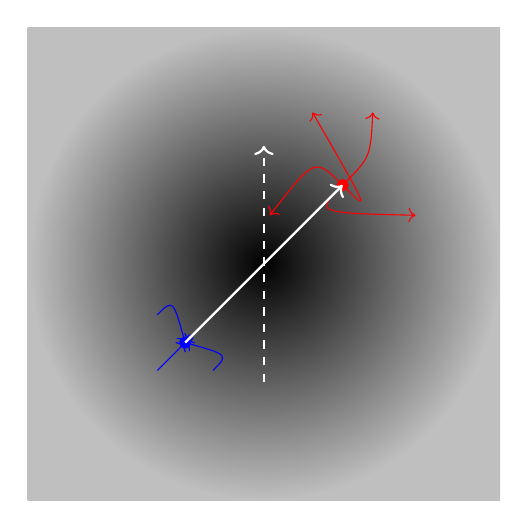
\begin{tikzpicture}
        % 定义背景渐变(类似黑洞的视觉效果)
        \shade[inner color=black, outer color=gray!50] (-3,-3) rectangle (3,3);
    
        % 绘制汇(Sink),位于较低位置
        \filldraw[blue] (-1, -1) circle (2pt) node[below left] {汇};
        \foreach \angle in {45,135,225,315} {
            \draw[blue, ->] (\angle:0.5) ++(-1,-1) .. controls +(0.2,0.2) .. (-1,-1);
        }
    
        % 绘制源(Source),位于较高位置
        \filldraw[red] (1, 1) circle (2pt) node[above right] {源};
        \foreach \angle in {45,135,225,315} {
            \draw[red, ->] (1,1) .. controls +(\angle:0.5) .. +(1.5*\angle:1);
        }
    
        % 绘制流线,从汇指向源
        \draw[thick, ->, white] (-1,-1) -- (1,1) node[midway, above right] {流方向};
    
        % 绘制高度方向
        \draw[thick, dashed, ->, white] (0,-1.5) -- (0,1.5) node[above, left] {高度};
    \end{tikzpicture}
\end{add}
\section{class 20}
期中考试,略……
\section{class 21}
\begin{defn}

    \textbf{Wake(涡流或纹路)}是流体在流动过程中由于流动不均匀或外界干扰而形成的旋转流动区域,通常表现为纹路或涡流现象。
    \begin{itemize}
        \item \textbf{Lifting Wake(升力纹路)}:由飞机机翼产生的升力引起的纹路现象,通常发生在飞机起飞或降落时。
        \item \textbf{Viscous Wake(粘性涡流)}:由流体的粘性效应引起的涡流现象,常见于流体流过粗糙表面或障碍物时。
        \item \textbf{Hydrodynamic Wake(流动力学涡流)}:由流体流动与外界环境(如水流、空气流或地形)相互作用形成的涡流现象。
        \item \textbf{Atmospheric Wake(大气涡流)}:在大气中,由风暴或气流运动形成的涡流现象。
    \end{itemize}
\end{defn}
\begin{proposition}
  
    \(\vec{\vec{\epsilon}}_{ijk}\vec{\vec{\epsilon}}_{jkl} = 2\delta_{il}\)
    \begin{tui}
    首先,考虑 Levi-Civita 符号的乘积 \(\vec{\vec{\epsilon}}_{ijk}\vec{\vec{\epsilon}}_{jkl}\),其中 \(j\) 和 \(k\) 是求和指标。
    
    根据 Levi-Civita 符号的性质,我们有:
    \[
    \vec{\vec{\epsilon}}_{ijk}\vec{\vec{\epsilon}}_{jkl} = \sum_{j,k} \vec{\vec{\epsilon}}_{ijk}\vec{\vec{\epsilon}}_{jkl}
    \]
    
    利用 Levi-Civita 符号的乘积公式:
    \[
    \vec{\vec{\epsilon}}_{ijk}\vec{\vec{\epsilon}}_{jkl} = \delta_{il}\delta_{kk} - \delta_{ik}\delta_{kl}
    \]
    
    其中 \(\delta_{kk}\) 是 Kronecker delta 的迹,对于三维空间,\(\delta_{kk} = 3\)。
    
    因此,上式可以简化为:
    \[
    \vec{\vec{\epsilon}}_{ijk}\vec{\vec{\epsilon}}_{jkl} = \delta_{il} \cdot 3 - \delta_{ik}\delta_{kl}
    \]

    注意到 \(\delta_{ik}\delta_{kl} = \delta_{il}\),    
    因此:
    \[
    \vec{\vec{\epsilon}}_{ijk}\vec{\vec{\epsilon}}_{jkl} = 3\delta_{il} - \delta_{il} = 2\delta_{il}
    \]
\end{tui}
\end{proposition}
\begin{lemma}
    在三维空间中,Levi-Civita 符号的乘积公式为:
\begin{align*}
    \vec{\vec{\epsilon}}_{ijk}\vec{\vec{\epsilon}}_{lmn} &= 
    \begin{vmatrix}
    \delta_{il} & \delta_{im} & \delta_{in} \\
    \delta_{jl} & \delta_{jm} & \delta_{jn} \\
    \delta_{kl} & \delta_{km} & \delta_{kn}
    \end{vmatrix}\\
    &=\delta_{il}\delta_{jm}\delta_{kn} - \delta_{il}\delta_{jn}\delta_{km} - \delta_{im}\delta_{jl}\delta_{kn} 
    + \delta_{im}\delta_{jn}\delta_{kl} + \delta_{in}\delta_{jl}\delta_{km} - \delta_{in}\delta_{jm}\delta_{kl}     
\end{align*}
\end{lemma}
\begin{corollary}

    if $i=l,j\neq m,k\neq n$ ,
    \begin{align*}
        \vec{\vec{\epsilon}}_{ijk}\vec{\vec{\epsilon}}_{lmn}
        &=\delta_{ii}\delta_{jm}\delta_{kn} - \delta_{ii}\delta_{jn}\delta_{km} - \delta_{im}\delta_{ji}\delta_{kn} 
        + \delta_{im}\delta_{jn}\delta_{ki} + \delta_{in}\delta_{ji}\delta_{km} - \delta_{in}\delta_{jm}\delta_{ki}
        \\&=3\left(\delta_{jm}\delta_{kn} - \delta_{jn}\delta_{km}\right)-\delta_{jm}\delta_{kn}+\delta_{km}\delta_{jn}
        +\delta_{jn}\delta_{km}-\delta_{kn}\delta_{jm}
        \\&=\delta_{jm}\delta_{kn} - \delta_{jn}\delta_{km}
    \end{align*}
    if $i=l,j=m,k\neq n$ ,
    \[
        \vec{\vec{\epsilon}}_{ijk}\vec{\vec{\epsilon}}_{lmn}
        =\delta_{jm}\delta_{kn} - \delta_{jn}\delta_{km}
        =\delta_{jj}\delta_{kn} - \delta_{jn}\delta_{kj}
        =2\delta_{kn}
    \]
    if $i=l,j=m,k=n$ ,
    \[
        \vec{\vec{\epsilon}}_{ijk}\vec{\vec{\epsilon}}_{lmn}
        =\vec{\vec{\epsilon}}_{ijk}\cdot\vec{\vec{\epsilon}}_{ijk}
        =2\delta_{kk}=3!=6
    \]
\end{corollary}
\begin{example}
    二倍的关系:$\vec{\Omega}=2\vec{\omega}$
\begin{flushleft}
    其中:
    \begin{itemize}
        \item $\vec{\Omega}$是涡量
        \item $\vec{\omega}$是角速度
    \end{itemize}
\end{flushleft}

1.error in beauty——Arnold Sommerfeld

Thus we cannot but offer an apology in reference to this defect

2.unfortunate factor——batchelor

\end{example}
\begin{defn}
    三维streamline coordinate流线坐标系

\begin{tikzpicture}[>=Stealth, scale=1.5, line join=round, line cap=round]

    % 定义更弯曲的流线(三维曲线)
    \draw[thick, ->] plot[smooth, tension=0.5] coordinates {
        (0,0,0) (1,1.5,1.5) (2,1,1) (3,1.5,1.5) (4,2,0)
    } node[right] {流线};

    % 定义切线方向(s方向)
    \draw[->, thick, red] (2,1,1) -- ++(0.7,0.35,0.35) node[above] {$\vec{\tau}$};
    \draw[dashed, red] (2,1,1) ++(0.7,0.35,0.35) -- ++(0.3,0.15,0.15);

    % 定义法线方向(n方向)
    \draw[->, thick, blue] (2,1,1) -- ++(-0.2,0.5,-0.2) node[left] {$\vec{n}$};
    \draw[dashed, blue] (2,1,1) ++(-0.2,0.5,-0.2) -- ++(-0.1,0.25,-0.1);

    % 定义副法线方向(b方向)
    \draw[->, thick, green!60!black] (2,1,1) -- ++(-0.3,-0.2,0.6) node[above right] {$\vec{b}$};
    \draw[dashed, green!60!black] (2,1,1) ++(-0.3,-0.2,0.6) -- ++(-0.15,-0.1,0.3);

    % 标注点
    \filldraw (2,1,1) circle (1.5pt) node[below right] {$P$};

    % 绘制三维坐标系
    \draw[->, thick] (0,0,0) -- (5,0,0) node[right] {$x$};
    \draw[->, thick] (0,0,0) -- (0,3,0) node[above] {$y$};
    \draw[->, thick] (0,0,0) -- (0,0,2) node[below left] {$z$};

\end{tikzpicture}
\begin{itemize}
    \item tangent $\vec{\tau}=\frac{d\vec{r}}{ds}$
    \item principal normal $\vec{n}=R\frac{d\vec{\tau}}{ds}$,scale factor$R=radius\, of\, curvature$
    \item binormal $\vec{b}=\vec{\tau}\times\vec{n}$
    \item osculating plane
    \item normal plane
    \item rectifying plane
\end{itemize}
\end{defn}
\begin{example}
    
    $\vec{v}=v\vec{\tau}$,
    $\vec{\Omega}=\nabla\times\vec{v}=
        \begin{vmatrix}
        \vec{\tau} & \vec{n} & \vec{b} \\
        \frac{\partial}{\partial\tau} & \frac{\partial}{\partial n} & \frac{\partial}{\partial b} \\
        v & 0 & 0
        \end{vmatrix}
        =\frac{\partial v}{\partial b}\vec{n}-\frac{\partial v}{\partial n}\vec{b}
        $
\end{example}
\begin{defn}

    在三维streamline coordinate流线坐标系中
    \begin{align*}
        \Omega_t&=\left(\vec{\tau}\cdot\nabla\times\vec{\tau}\right)v\\
            \Omega_n&=\frac{\partial v}{\partial b}\\
            \Omega_b&=\frac{v}{R}-\frac{\partial v}{\partial n}
    \end{align*}
\end{defn}
\begin{example}
    \[
        2\omega=\Omega_b=\underbrace{\frac{v}{R}}_{\omega}
        -\underbrace{\frac{\partial v}{\partial n}}_{-\frac{\partial v}{\partial r}=-\omega}
    \]
\end{example}
\begin{example}
    点涡流$V=\frac{\Gamma}{2\pi r}$
    \[
    \Omega_b=\frac{\Gamma}{2\pi r^2}-\frac{\Gamma}{2\pi r^2}=0
    \]
\end{example}
\section{class 22}
\begin{proposition}
\[
\text{兰姆矢量形式的矢量恒等式}\vec{L}=\left(\nabla\times\vec{v}\right)\times\vec{v}
=\vec{v}\cdot\nabla\vec{v}-\nabla\left(\frac{1}{2}\vec{v}^2\right)
\]
\begin{proof}
    \begin{align*}
        \vec{L}&=\left(\left(\frac{\partial}{\pa x_i}\vec{e_i}\right)\times
        \left(v_j\vec{e_j}\right)\times\left(v_k\vec{e_k}\right)\right)\\
        &=\frac{\pa}{\pa x_i}\left(v_j\vec{\vec{\epsilon}}_{ijl}\vec{e_l}\right)\times\left(v_k\vec{e_k}\right)\\
        &=\frac{\pa v_jv_k}{\pa x_i}\vec{\vec{\epsilon}}_{ijl}\vec{\vec{\epsilon}}_{lkm}\vec{e_m}\\
        &=\frac{\pa v_j}{\pa x_i}v_i\vec{e_j}-\frac{\pa v_j}{\pa x_j}v_j\vec{e_i}\\
        &=\vec{v}\cdot\nabla\vec{v}-\nabla\left(\frac{1}{2}\vec{v}^2\right)
    \end{align*}
\end{proof}
\end{proposition}
\begin{proposition}
    \[
    \nabla\cdot\left(\vec{a}\times\vec{b}\right)
    =\vec{b}\cdot\left(\nabla\times\vec{a}\right)-\vec{a}\cdot\left(\nabla\times\vec{b}\right)
    \]
    \begin{proof}
        \begin{align*}
            \nabla\cdot\left(\vec{a}\times\vec{b}\right)
            &=\left(\frac{\pa}{\pa x_i}\vec{e_i}\right)\cdot
            \left(a_jb_k\vec{\vec{\epsilon}}_{jkl}\vec{e_k}\right)\\
            &=\frac{\pa}{\pa x_i}\left(a_jb_k\vec{\vec{\epsilon}}_{jkl}\delta_{il}\right)\\
            &=\frac{\pa a_j}{\pa x_i}b_k\vec{\vec{\epsilon}}{jki}+a_j\frac{\pa b_k}{\pa x_i}\vec{\vec{\epsilon}}{jki}\\
            &=b_k \left( \nabla \times \vec{a} \right)_k +\vec{a} \cdot \left( \nabla \times \vec{b} \right)\\
            &=\vec{b}\cdot\left(\nabla\times\vec{a}\right)-\vec{a}\cdot\left(\nabla\times\vec{b}\right)
        \end{align*}
    \end{proof}
\end{proposition}
\begin{proposition}
    \[
    \nabla\times\left(\varphi\vec{a}\right)=\varphi\left(\nabla\times\vec{a}\right)
    +\left(\nabla\varphi\right)\times\vec{a}
    \]
    \begin{proof}
        \begin{align*}
            \nabla\times\left(\varphi\vec{a}\right)
            &=\left(\frac{\pa}{\pa x_i}\vec{e_i}\right)\times\left(\varphi a_j\vec{e_j}\right)\\
            &=\frac{\pa}{\pa x_i}\left(\varphi a_j\vec{\vec{\epsilon}}_{ijk}\vec{e_k}\right)\\
            &=\frac{\pa \varphi}{\pa x_i}a_j\vec{\vec{\epsilon}}_{ijk}\vec{e_k}
            +\varphi\frac{a_j}{x_i}\vec{\vec{\epsilon}}_{ijk}\vec{e_k}\\
            &=\varphi\left(\nabla\times\vec{a}\right)+\left(\nabla\varphi\right)\times\vec{a}
        \end{align*}
    \end{proof}
\end{proposition}
\begin{proposition}
    \[
    \nabla\times\left(\vec{a}\times\vec{b}\right)=
    \vec{b}\cdot\nabla\vec{a}-\vec{a}\cdot\nabla\vec{b}+
    \vec{a}\left(\nabla\cdot\vec{b}\right)-\vec{b}\left(\nabla\cdot\vec{a}\right)
    \]
    \begin{proof}
        \begin{align*}
            \nabla\times\left(\vec{a}\times\vec{b}\right)
            &=\left(\frac{\pa}{\pa x_i}\vec{e_i}\right)\times\left(a_jb_k\vec{\vec{\epsilon}}_{jkm}\vec{e_m}\right)\\
            &=\frac{\pa}{\pa x_i}\left(a_jb_k\vec{\vec{\epsilon}}_{jkm}\vec{\vec{\epsilon}}_{imn}\vec{e_n}\right)
            =\frac{\pa}{\pa x_i}\left(a_jb_k\right)\vec{\vec{\epsilon}}_{jkm}\vec{\vec{\epsilon}}_{imn}\vec{e_n}\\
            &=\left(\frac{\pa a_i}{\pa x_i}b_k+\frac{\pa b_k}{\pa x_i}a_j\right)\left(\delta_{jn}\delta_{ki}-\delta_{kn}\delta_{ji}\right)\vec{e_n}\\
            &=\underbrace{\frac{\pa a_j}{\pa x_i}b_i\vec{e_j}}_{\vec{b}\cdot\nabla\vec{a}}
            -\underbrace{\frac{\pa b_k}{\pa x_i}a_i\vec{e_k}}_{\vec{a}\cdot\nabla\vec{b}}
            +\underbrace{\frac{\pa b_i}{\pa x_i}a_j\vec{e_j}}_{\vec{a}\left(\nabla\cdot\vec{b}\right)}
            -\underbrace{\frac{\pa a_i}{\pa x_i}b_k\vec{e_k}}_{\vec{b}\left(\nabla\cdot\vec{a}\right)}
        \end{align*}
    \end{proof}
\end{proposition}
\begin{proposition}
    \[
    \nabla\times\left(\nabla\times\vec{a}\right)=\nabla\left(\nabla\cdot\vec{a}\right)-\nabla^2\vec{a}
    \]
    \begin{proof}
        \begin{align*}
            (\nabla \times (\nabla \times \vec{a}))_i&= \vec{\vec{\epsilon}}_{ijk} \frac{\pa}{\pa x_j} (\nabla \times \vec{a})_k
            = \vec{\vec{\epsilon}}_{ijk} \vec{\vec{\epsilon}}_{klm} \frac{\pa^2}{\pa x_jx_l}  a_m\\
            &=\frac{\pa^2}{\pa x_ix_j} a_j - \frac{\pa^2}{\pa x_j^2} a_i
            =\nabla (\nabla \cdot \vec{a}) - \nabla^2 \vec{a}
        \end{align*}
    \end{proof}
\end{proposition}











%  ↑↑↑↑↑↑↑↑↑↑↑↑↑↑↑↑↑↑↑↑↑↑↑↑↑↑↑↑ 正文部分
\ifx\allfiles\undefined
\end{document}
\fi
